% To compile:
%  pdflatex design

\documentclass[11pt]{article}

\usepackage[titles]{tocloft}
\usepackage{verbatim}
\usepackage[pdftex]{graphics,graphicx}
\usepackage{float}
\usepackage{mathtools}
\usepackage{amssymb}
\usepackage{hyperref}
\usepackage{appendix}
\usepackage{listings}
\usepackage{color}
\usepackage{pmboxdraw}

% pdf stuff
\hypersetup{
  pdfauthor={Geoff Johnson},
  pdftitle={Network Security},
  pdfsubject={Honeynet Project Design},
  pdfkeywords={COMP8506 Honeynet Project},
  colorlinks=true,
  linkcolor=black,
  urlcolor=blue
}

% salmon on ice color scheme from kuler
\definecolor{soi-basic}{RGB}{62,69,76}
\definecolor{soi-comment}{RGB}{255,127,102}
\definecolor{soi-keyword}{RGB}{33,133,197}
\definecolor{soi-string}{RGB}{126,206,253}
\definecolor{soi-background}{RGB}{255,246,229}

% default margins are too wide all the way around, reset them
\setlength{\topmargin}{-.5in}
\setlength{\textheight}{9in}
\setlength{\oddsidemargin}{0in}
\setlength{\textwidth}{6.5in}

% change paragraph formatting
\setlength{\parindent}{0pt}
\setlength{\parskip}{2ex}

\lstset{
  language=bash,
  backgroundcolor=\color{soi-background},
  identifierstyle=\ttfamily,
  basicstyle=\footnotesize\ttfamily\color{soi-basic},
  keywordstyle=\color{soi-keyword},
  commentstyle=\color{soi-comment},
  stringstyle=\color{soi-string},
  tabsize=4,
  aboveskip={1.5\baselineskip},
  columns=fixed,
  inputencoding=utf8,
  extendedchars=true,
  breaklines=true,
  prebreak = \raisebox{0ex}[0ex][0ex]{\ensuremath{\hookleftarrow}},
  frame=single,
  showtabs=false,
  showspaces=false,
  showstringspaces=false,
  numbers=left,
  numberstyle=\tiny,
  breakatwhitespace=true,
  title=\lstname,
  literate={│}{{\textSFxi}}1 {└}{{\textSFii}}1 {├}{{\textSFviii}}1 {─}{{\textSFx}}1,
}

% add commands to handle some common superscripts in text mode
\newcommand{\superscript}[1]{\ensuremath{^{\textrm{#1}}}}
\newcommand{\subscript}[1]{\ensuremath{_{\textrm{#1}}}}
%\newcommand{\th}[0]{\superscript{th}}
%\newcommand{\st}[0]{\superscript{st}}
%\newcommand{\nd}[0]{\superscript{nd}}
%\newcommand{\rd}[0]{\superscript{rd}}

\begin{document}
\nocite{*}

  % title page
  \title{
    Honeynet Design
  }
  \author{
    Geoff Johnson ... \\
    A00533481 ... \\ \\
    COMP8506
  }
  \renewcommand{\today}{April xx, 2013}
  \maketitle
  \thispagestyle{empty}
  \newpage
  \mbox{}
  \thispagestyle{empty}

  \newpage
  \addtocounter{page}{-1}
  \pagenumbering{roman}
  \tableofcontents
  \listoffigures
  \listoftables
  \lstlistoflistings

  \newpage
  \pagenumbering{arabic}

  % abstract
  \section{Abstract}
    \label{sec:abstract}

    Abstract goes here ...

  \section{Introduction}
    \label{sec:intro}

    Introduction goes here ...

  \newpage
  \section{Design}
    \label{sec:dsg}

    Design description ...

    \subsection{Network}
      \label{sec:dsg_net}

      Network layout description ...

      % Sample figure
      \begin{figure}[H]
        \centering
        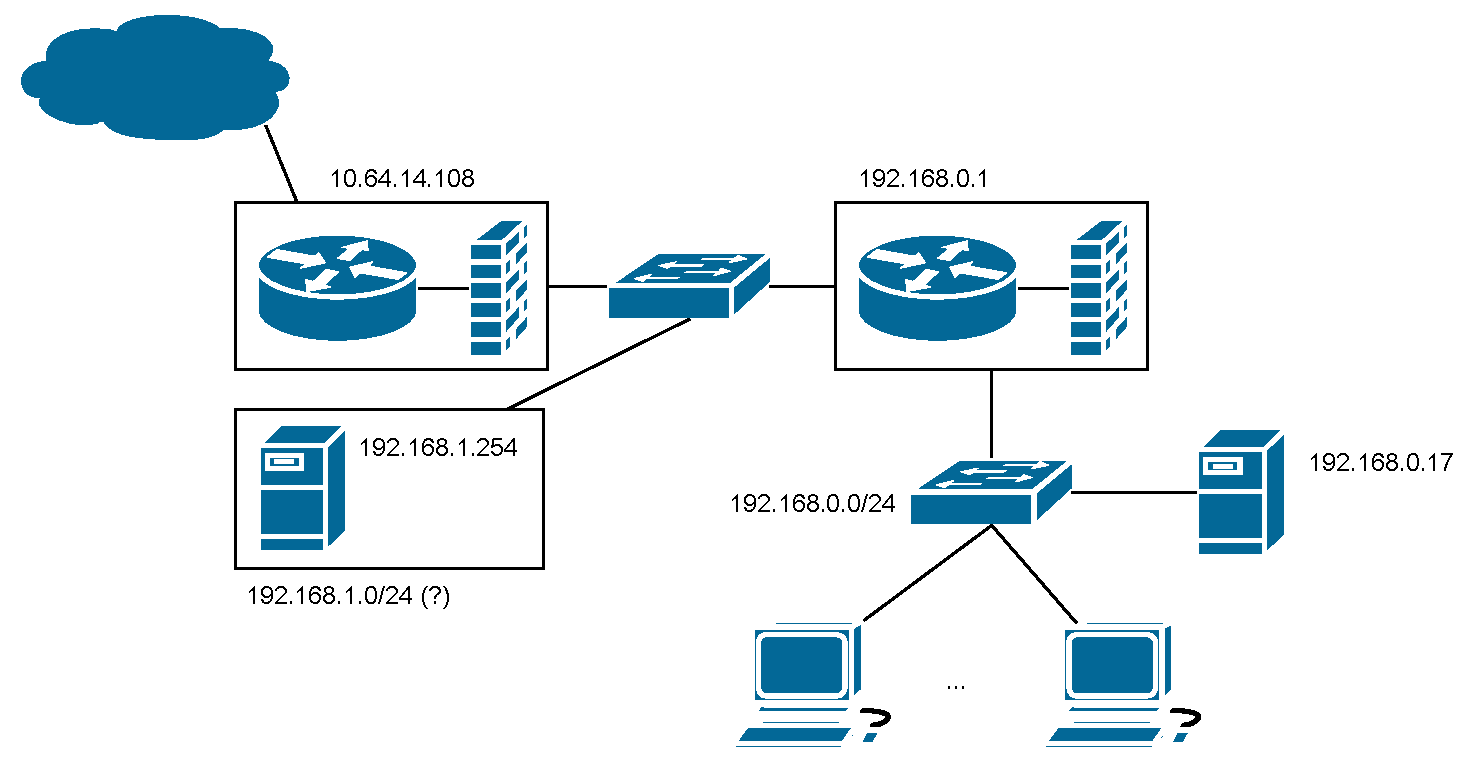
\includegraphics[scale=.6]{figures/network-diagram.pdf}
        \caption{Network Diagram}
        \label{fig:dsg_net:diagram}
      \end{figure}

  \section{Collection}

    % Sample listing
    \begin{lstlisting}[caption={Collecting Data},
                       label={lst:collect_data}]
#!/bin/bash
tcpdump -i eth0 -o /var/log/captures/tcpdump-`date +%Y-%m-%d`.pcap
    \end{lstlisting}

    \subsection{Tools}
      \label{sec:tools}

      Several tools will be used to acquire log data etc... such as:

      \begin{itemize}
        \item bash, perl
        \item tcpdump
        \item snort
      \end{itemize}

  % appendices
  \newpage
  \addappheadtotoc
  \appendix
  \appendixpage

  \section{Scripts Used to Do Stuff}
    \label{app:scripts}

    \subsection{Backing Up Linux Hosts}
      \label{app:scripts:backup}

      \lstinputlisting[caption={Script to Backup Linux Host Logs and Packet Captures},
                       label={lst:scripts:backup}]
        {../scripts/backup.sh}

\end{document}

%% vim: set expandtab ts=2 sw=4: %%
